\documentclass[12pt]{article}
\usepackage{graphicx}
\begin{document}

\title{Title}

\section*{Brain Challenge}

This project aim to analyze the relationship between a bunch of features computed on several NRM images of the brain of different patients and the age of those patients. The final purpose of this analysis is to attempt to detect those images' features that are better able to predict the patient's age and try to extract the biological meaning from this information.

The raw images database had already been pre-processed when it was sent to me. Therefore my work started with a dataframe with about 1000 features collected on almost 2000 samples (\texttt{n\_features} = 954 and \texttt{n\_samples} = 2631?).


\subsection*{Dimensionality Reduction}
The reduction in the number of features is one of the key point of this analysis. I wanted to conserve the meaning of each features in the reduced space so I avoided the use of any dimensionality reduction method that worked with a combination of features as PCA or ???. What I've looked for was a method to score the importance of any feature in the prediction of the age of the subject. Hence I used different combinations of scaler method, to standardize the data, and penalized linear model like ridge, Lasso and the elastic net. The coefficients of theese regressions have been used as scores in the determination of which were the most predictive features.

More precisely, I used three different method to standardize the data: the \texttt{MinMaxScaler}, the \texttt{StandardScaler} and the \texttt{RobustScaler}. The \texttt{MinMaxScaler} scales the each feature individually to the range $\lbrack 0,1 \rbrack$, and it's the one that received the best scores among the three. The \texttt{StandardScaler} modify each single column simply setting the mean to 0 and the standard deviation to 1. The \texttt{RobustScaler} instead manage every feature giving less importance to outliers.

Those scaling methods were combined with three penalized regression methods: the \texttt{LassoCV}, the \texttt{RidgeCV}, and the \texttt{ElasticNetCV}.All these three supervised methods are linear in the coefficients, and what you obtain after such a regression is the array of values that express the linear combination of features that better predict the age of the samples. Every one of these methods find the best hyper-parameters for the regression and perform automatically a cross validation on their results.  The Lasso regression exerts a penalization on the L1-norm of the coefficients vector, the ridge regression instead is based on the L2-norm of the vector, while the elastic net method performs a sort of mixture of the two methods.

The total number of combinations among these elements is nine. So I processed the data with each one of them and obtained nine arrays of coefficients. Then I was able to sort the absolute values of those coefficients in order to find the most important ones for every combination. The idea was to select a certain number of the most influential features and use them to perform further analysis.

\begin{figure}
  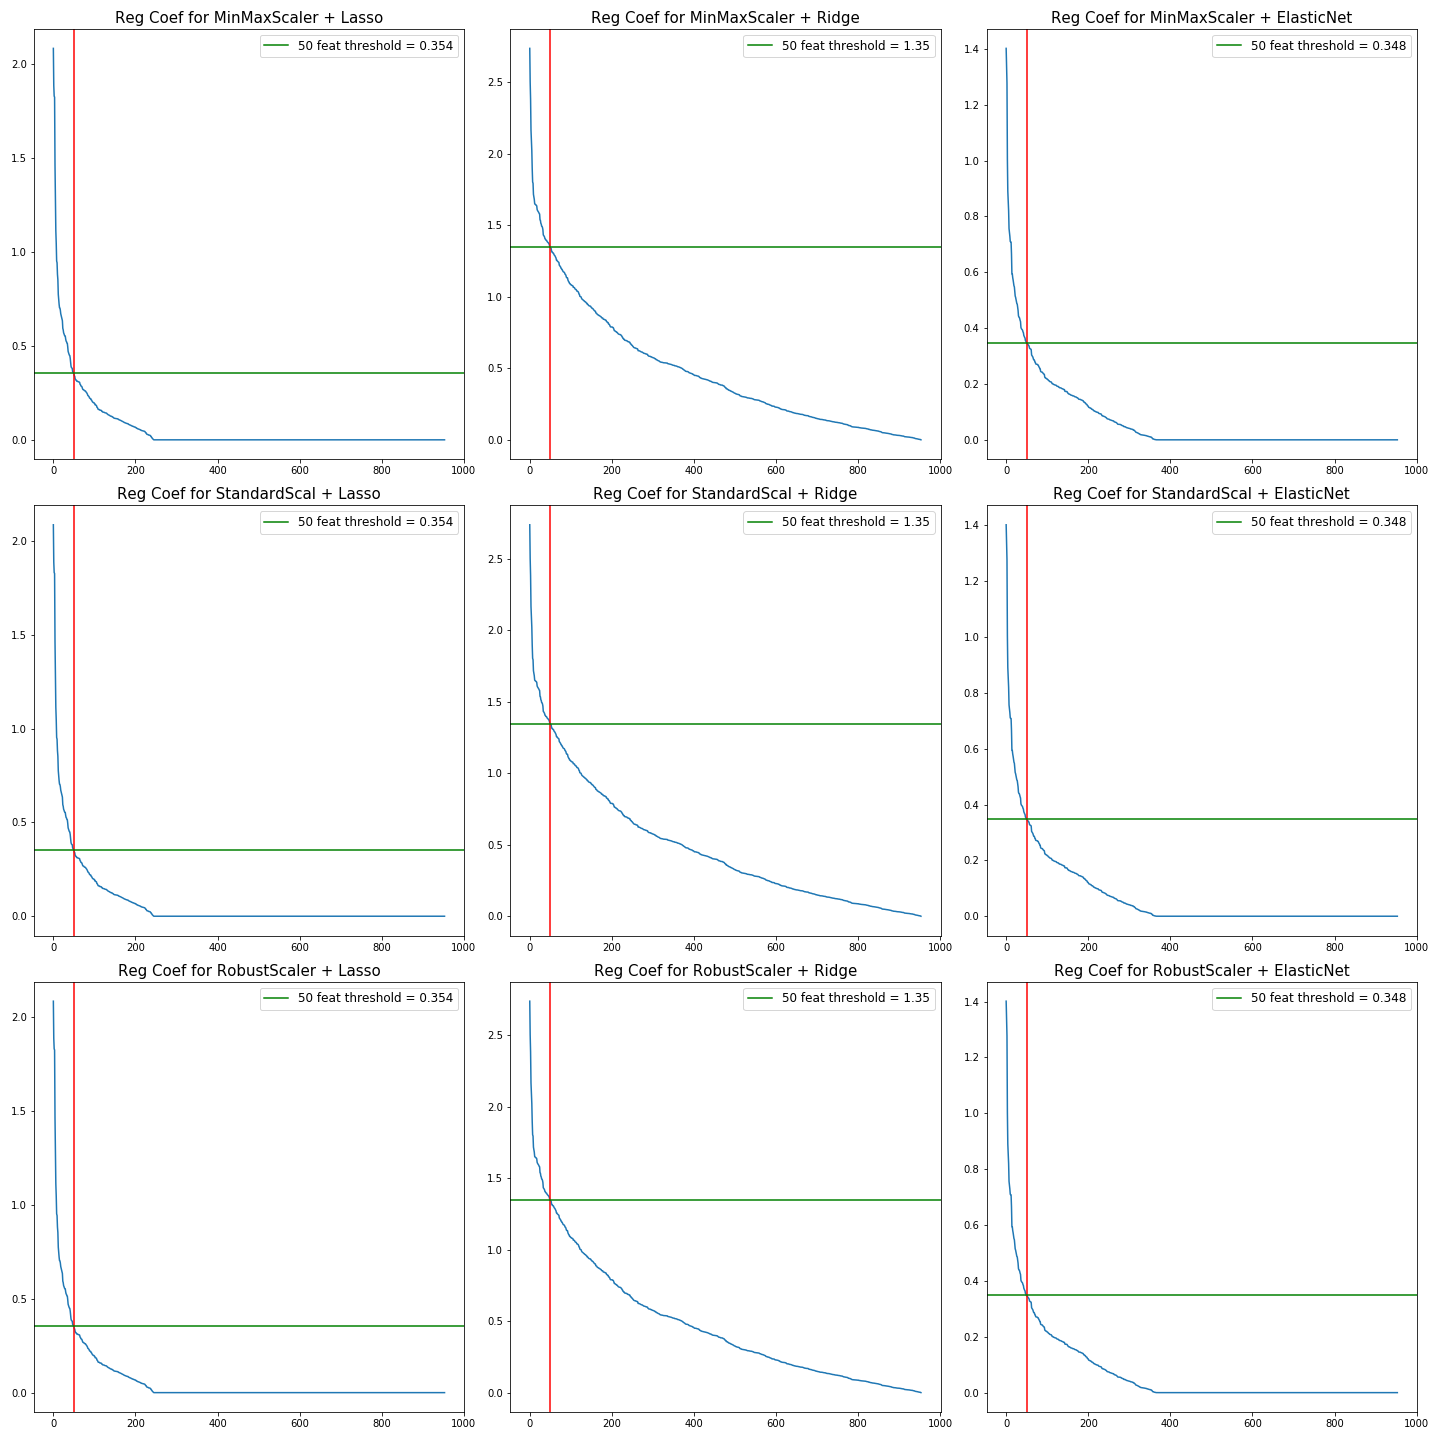
\includegraphics[width=\linewidth]{NineCoefPlot.png}
  \caption{The nine plots that shows the general trend for each one of the scaler + regression combinations. It can be seen that they behave quite the same way. The threshold value does not change at all varying the scaler method, but it depends clearly on the regression method. The vertical red line identify the 50 highest ranked features, while the green horizontal line highlight the threshold value necessary to filter only those features.}
  \label{fig:boat1}
\end{figure}





\end{document}
